\chapter{PREDICTIVE FOREST}
\label{sect:pforest}
Predictive forest is a novel data structure supports predictive queries over road networks given that users' location is imprecise. There are two building block algorithms for the \pf data structure described in the upcoming sections.

\section {Building \PF}
The algorithm is given the road network $G=\{N,E,W\}$, a time range $\cal T$, a starting region $r$ which consists of center node $n$ and radius $d$ as input. After that the algorithm start execution by the following:
\begin{itemize}
    \item {\bf Roots Extraction.} The input region is processed to extract all the nodes inside that region with the specific radius. The outcome of this step are the roots of the forest.
    \item {\bf Building \PT.} For every root node, construct a \pt $Tree$ \cite{Hendawi15}
    \item {\bf \PT Integration.} Given the $Tree$ from previous step, merge it in the forest. There are multiple cases to mention here:
    \begin{itemize}
        \item The first $Tree$ to occur in the building algorithm is merged as is to the forest
        \item For every subsequent $Tree$, if a node $n_t$ from $Tree$ already exists in the forest as $n_f$ find out which one is closer to the forest roots and use then them remove that node along with its subtree and merge/keep the other one.
    \end{itemize}
    \item {\bf Probability Computation.} a breadth-first search algorithm is applied to the forest and every node is assigned probability $1/n$ where $n$ is the number of siblings. This will be described in detail in section ~\ref{sec:prob}.
\end{itemize}

The pseudo code for \pf building algorithm reveals the aforementioned steps in Algorithm ~\ref{alg:building}

\begin{algorithm} [ht]
\caption{Building \PF}
\label{alg:building}
\begin{footnotesize}
\textbf{Input:} $Region~R$, $Time~Range~\cal T$, Road Network Graph $G(N,E,W)$
\begin{algorithmic}[1]
\STATE \PF $PF \leftarrow \emptyset$
\STATE \COMMENT {Step 1. Roots Extraction}
\STATE Array $Roots \leftarrow GetRoots(R)$
\FOR { \textbf{each} node $root$ in Roots }
    \STATE \COMMENT {Step 2. Building \PT}
    \STATE \PT $PT \leftarrow ConstructPredictiveTree(root, T, G)$ 
    \FOR { \textbf{each} node $n_t$ in $PT$ }
        \STATE \COMMENT {Step 3. \PT Integration}
        \IF { $n_t$ does not exists in $PF$ }
            \STATE Insert $n_t \rightarrow PF$
        \ELSE
            \STATE \COMMENT{Find the equivalent node in the forest for $n_t$}
            \STATE node $n_f \leftarrow PF.GetNode(n_t)$
            \STATE \COMMENT {Find out which node is closer to the forest roots}
            \IF { $n_t$ closer to $PF.Roots$ than $n_f$ }
                \STATE Remove subtree of $n_f \rightarrow PF$
                \STATE Remove $n_f \rightarrow PF$
            \ELSE
                \STATE Remove subtree of $n_t \rightarrow PT$
                \STATE Remove $n_t \rightarrow PT$
            \ENDIF
        \ENDIF
    \ENDFOR
\ENDFOR

\COMMENT {Step 4. Probability Computation}
\FOR {\textbf{each} node $n$ in $PF$}
    \STATE $n.Probability \leftarrow ComputeProbability(n)$
\ENDFOR
\STATE Return $PF$
\end{algorithmic}
\end{footnotesize}
\end{algorithm}

An example describing this in action in Figure ~\ref{fig:building}

\begin{figure*}[ht]
\centering
\subfigure[Road Network]{
\vtop{\vskip0pt
\hbox{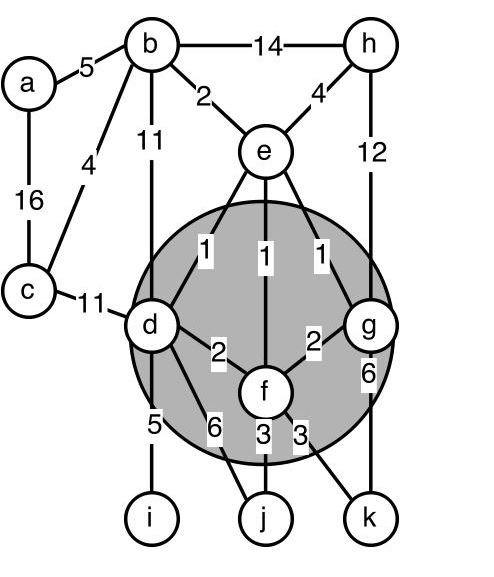
\includegraphics[scale = 0.285]{pf-build-1}}
}}
\subfigure[Adding root d tree]{
\vtop{\vskip0pt
\hbox{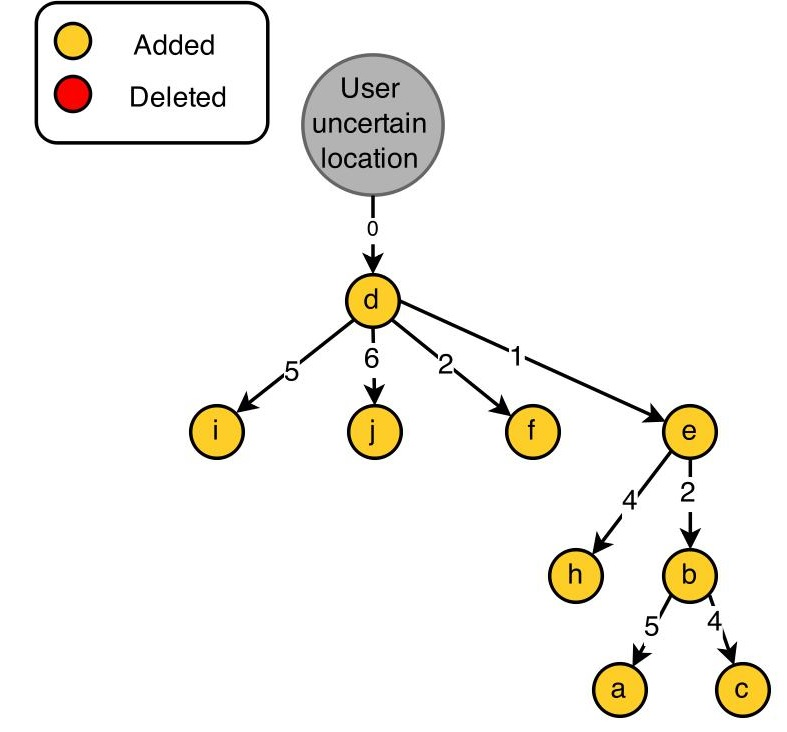
\includegraphics[scale = 0.285]{pf-build-2}}
}}
\subfigure[Adding root f tree]{
\vtop{\vskip0pt
\hbox{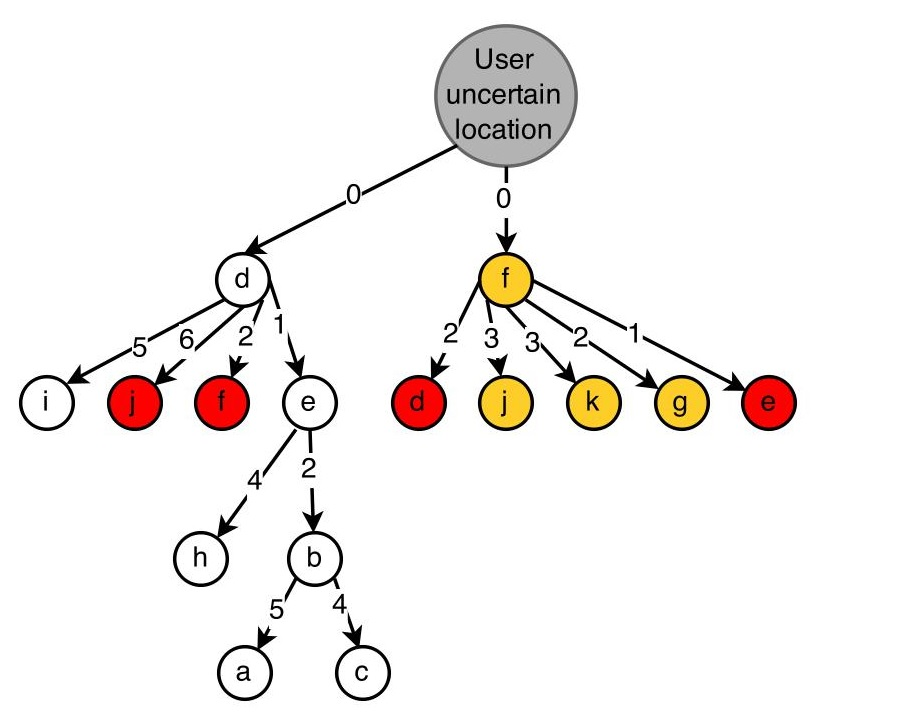
\includegraphics[scale = 0.285]{pf-build-3}}
}}
\\
\text \large \textcolor{red}{\textbf{\hl{TODO}}}: The nodes marked in red in the previous step (c) should
not be present in this graph at step (d), as they have been deleted by now! Hence, the nodes l, f, d, e, marked in red should be deleted from the graph for step (d).
\subfigure[Adding root g tree]{
\vtop{\vskip0pt
\hbox{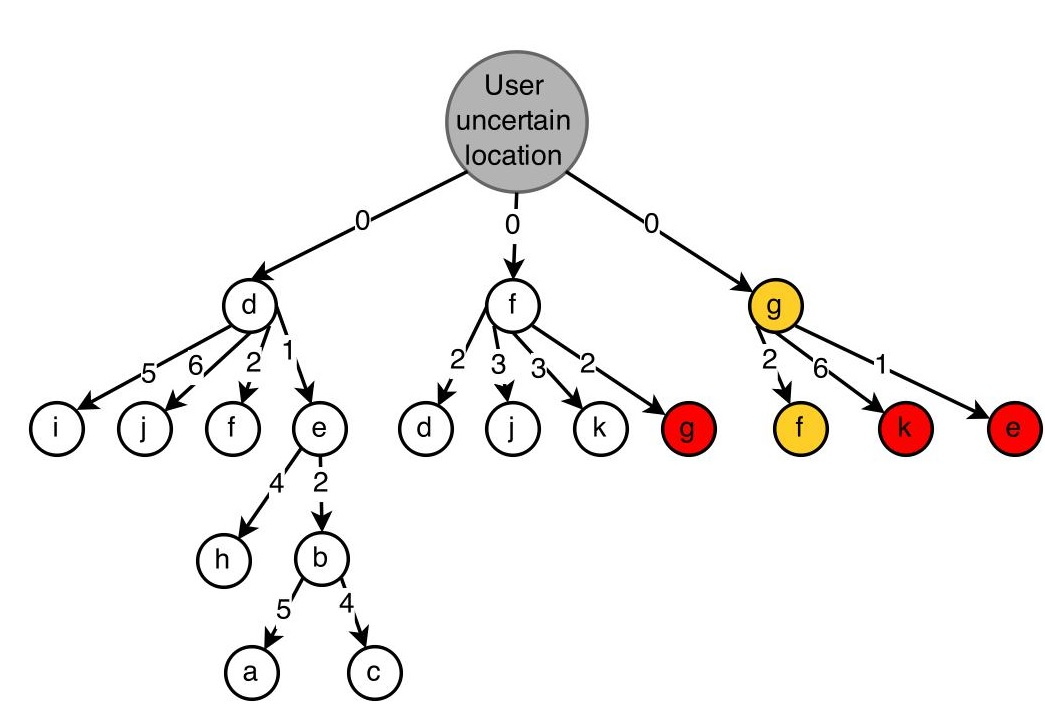
\includegraphics[scale = 0.285]{pf-build-4}}
}}
\caption{Building a \PF (better viewed in colored print)}
\label{fig:building}
\end{figure*}

\section {Updating \PF}
In the building phase the \pf has been constructed and in the update phase the \pf receives a new location for the user, mainly a new region and it predicts what is the next region the object will be at. This step works solely on the provided region plus the current history of the object. Moreover, normally in a road network objects seek the shortest path therefore \pf holds this assumption. The update algorithm steps are briefly summarized below given a region $r$ as input:
\begin{itemize}
    \item {\bf Roots Extraction.} The same algorithm used for extracting the roots is used in the update phase though the extracted nodes are passed to a next module to do further checking and pruning:
    \begin{itemize}
    \item First case, that all the extracted root nodes are found inside the tree already then they are treated as is and no pruning happens 
    \item Second case happens when some of the nodes appear in the existing \pf and some are new. In this case the out ranged roots (i.e. roots that are not in the \pf) are pruned from the extracted roots set to hold with the assumption that the object follows shortest path
    \item Third case is the one when all the extracted roots does not appear in the \pf which means that the object does not follow the shortest path assumption and in this case the existing \pf is destroyed and a newly \pf is build from the extracted roots set.
    \end{itemize}
    \item {\bf \PF Traversal.} For every root node in the extracted root nodes set, apply a breadth first search traversal algorithm to find out children of it and mark them as included node.
    \item {\bf \PF Pruning.} Starting from the existing roots for the \pf a breadth first search traversal algorithm is applied for every node in the forest. If the current node is marked as include keep it, otherwise prune it along with its subtree from the forest.
    \item {\bf Probability Computation.} Same probability computation algorithm applied in the \pf building step is applied here as well. This will be described in detail in section ~\ref{sec:prob}.
\end{itemize}

The pseudo code for \pf update algorithm mention in Algorithm ~\ref{alg:update}. In line ~\ref{l:subtree}:~\ref{alg:update} the input to the $Subtree$ is a node while the return is the subtree of it. The traversal algorithm in line ~\ref{l:dfs}:~\ref{alg:update} is necessary a depth-first search traversal to prune the leaves then got up until the root. This will make sure that an included node will not be deleted because on of it's ancestors is not included.

\begin{algorithm} [ht]
\caption{Updating \PF}
\label{alg:update}
\begin{footnotesize}
\textbf{Input:} $Region~R$, $Predictive~Forest~\cal PF$, $Time~Range~\cal T$, Road Network Graph $G(N,E,W)$
\begin{algorithmic}[1]
\STATE \COMMENT {Step 1. Roots Extraction}
\STATE Array $Roots \leftarrow GetRoots(R)$
\FOR { \textbf{each} node $root$ in Roots }
    \IF { $root$ does not exists in $PF$ }
        \STATE Remove node of $root \rightarrow Roots$
    \ENDIF
\ENDFOR

\IF { $Roots$ is empty }
    \STATE $PF \leftarrow FabricatePredictiveForest(R, T, G)$
\ELSE
    \STATE \COMMENT {Step 2. \PF Traversal}
    \STATE Hashtable $Included \leftarrow \emptyset$
    \FOR { \textbf{each} node $root$ in Roots }
    \STATE Insert $PF.GetSubtree(root) \rightarrow Included$ \label{l:subtree}
    \STATE Insert $root \rightarrow Included$
    \ENDFOR

\STATE \COMMENT {Step 3. \PF Pruning - Depth First Search Traversal}
\FOR { \textbf{each} node $n$ in $PF$ } \label{l:dfs}
\IF { $n$ does not exist in $Included$ }
    \STATE Remove subtree of $n \rightarrow PF$
    \STATE Remove $n \rightarrow PF$
\ENDIF
\ENDFOR

\COMMENT {Step 4. Probability Computation}
\FOR {\textbf{each} $n$ in $PF$ }
    \STATE $n.Probability \leftarrow ComputeProbability(n)$
\ENDFOR

\ENDIF

\STATE Return $PF$
\end{algorithmic}
\end{footnotesize}
\end{algorithm}

To aid the algorithm, an step-by-step example in ~\ref{fig:update} is provided for tracing an \pf update for an object.

\begin{figure*}[ht]
\centering
\subfigure[Road Network - Move 0]{
\vtop{\vskip0pt
\hbox{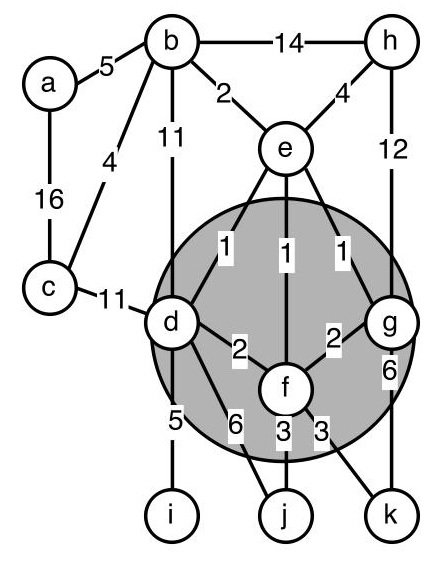
\includegraphics[scale = 0.285]{pf-update-1}}
}}
\subfigure[Predictive Forest - Move 0]{
\vtop{\vskip0pt
\hbox{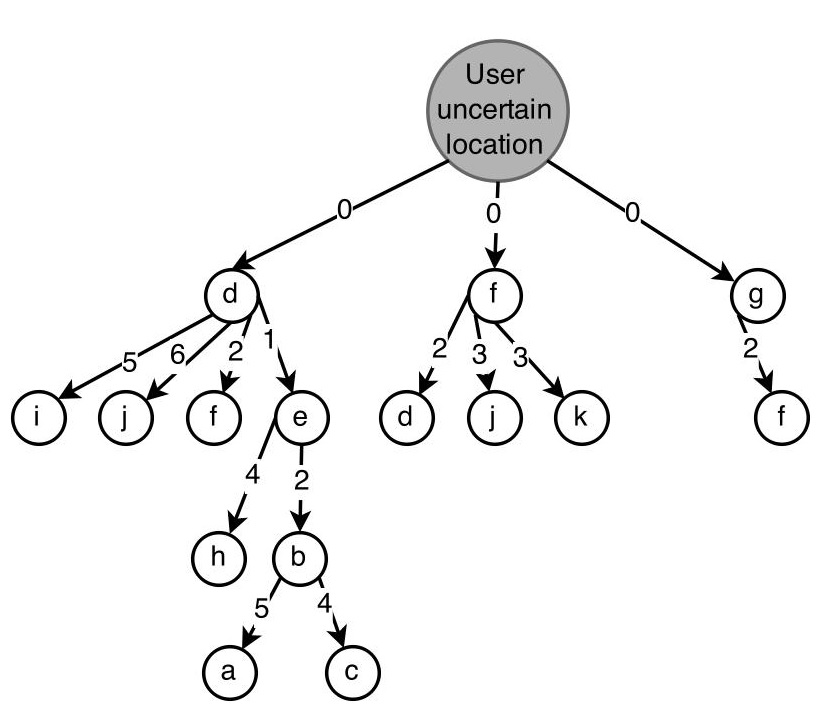
\includegraphics[scale = 0.285]{pf-update-2}}
}}
\\
\text \large \textcolor{red}{\textbf{\hl{TODO}}}: There are duplicate nodes
in this forest at Step (b) which is wrong. Please delete these nodes, recreate the 
graph and add it back here. The same applies to all other steps in this Figure.
\subfigure[Road Network - Move 1]{
\vtop{\vskip0pt
\hbox{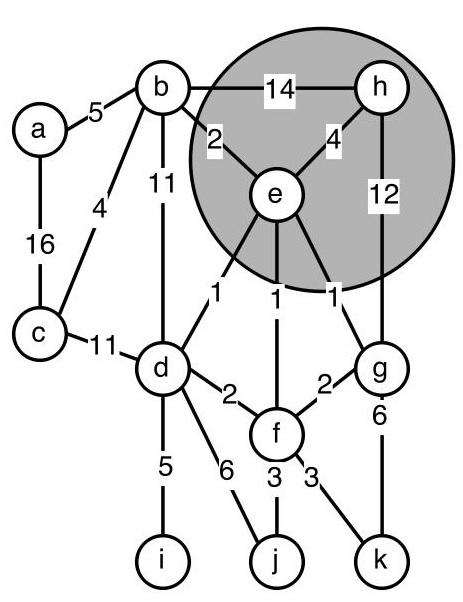
\includegraphics[scale = 0.285]{pf-update-3}}
}}
\subfigure[Predictive Forest - Move 1]{
\vtop{\vskip0pt
\hbox{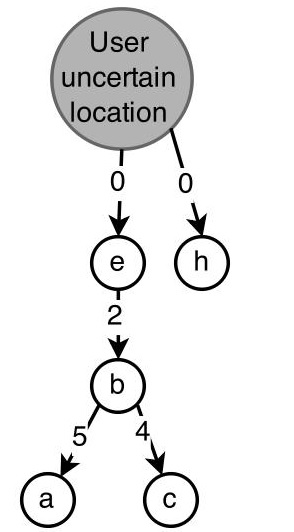
\includegraphics[scale = 0.285]{pf-update-4}}
}}
\subfigure[Road Network - Move 2]{
\vtop{\vskip0pt
\hbox{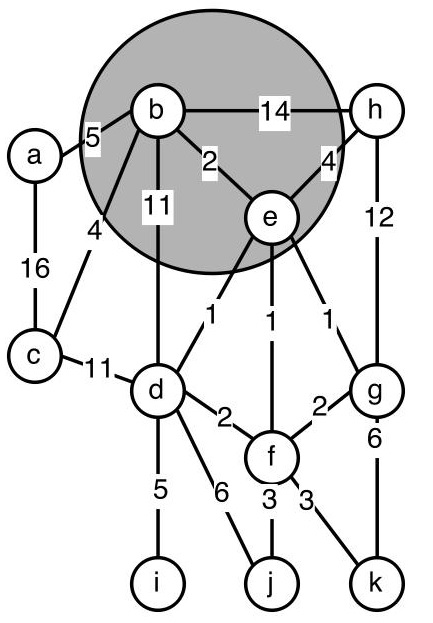
\includegraphics[scale = 0.285]{pf-update-5}}
}}
\subfigure[Predictive Forest - Move 2]{
\vtop{\vskip0pt
\hbox{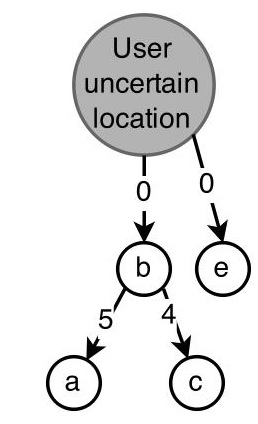
\includegraphics[scale = 0.285]{pf-update-6}}
}}
\subfigure[Road Network - Move 3]{
\vtop{\vskip0pt
\hbox{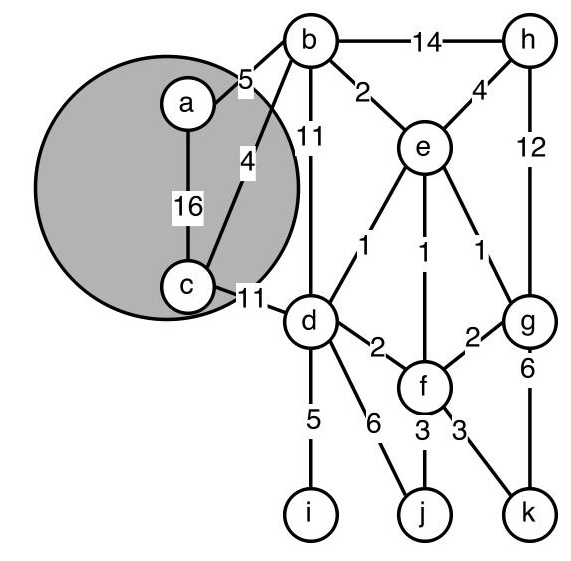
\includegraphics[scale = 0.285]{pf-update-7}}
}}
\subfigure[Predictive Forest - Move 3]{
\vtop{\vskip0pt
\hbox{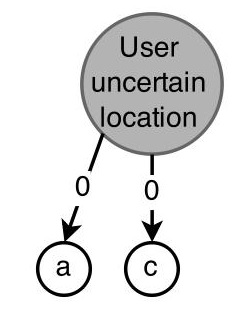
\includegraphics[scale = 0.285]{pf-update-8}}
}}
\caption{Updating a \PF}
\label{fig:update}
\end{figure*}

\section {Probability Computation}
\label{sec:prob}
In the previous sections the details of the probability computation was not revealed as there are many approaches to do that. Here we will describe one way of calculating the probabilities that we used in our experiments in Algorithm ~\ref{alg:prob}

\begin{algorithm} [ht]
\caption{Probability Computation}
\label{alg:prob}
\begin{footnotesize}
\textbf{Input:} $PredictiveForest~PF$
\begin{algorithmic}[1]
\FOR {\textbf{each} $node$ in $PF$}
    \STATE $sibilings \leftarrow PF.GetSiblings(node)$
    \STATE $node.Probability \leftarrow 1 / sibilings.Length$
\ENDFOR

\STATE Return $PF$
\end{algorithmic}
\end{footnotesize}
\end{algorithm}

The lookup for nodes in the forest is optimized by storing references to node keys into a hashtable that points to the actual node reference as show in figure ~\ref{fig:hashtable}

\begin{figure}[ht]
  \centering
    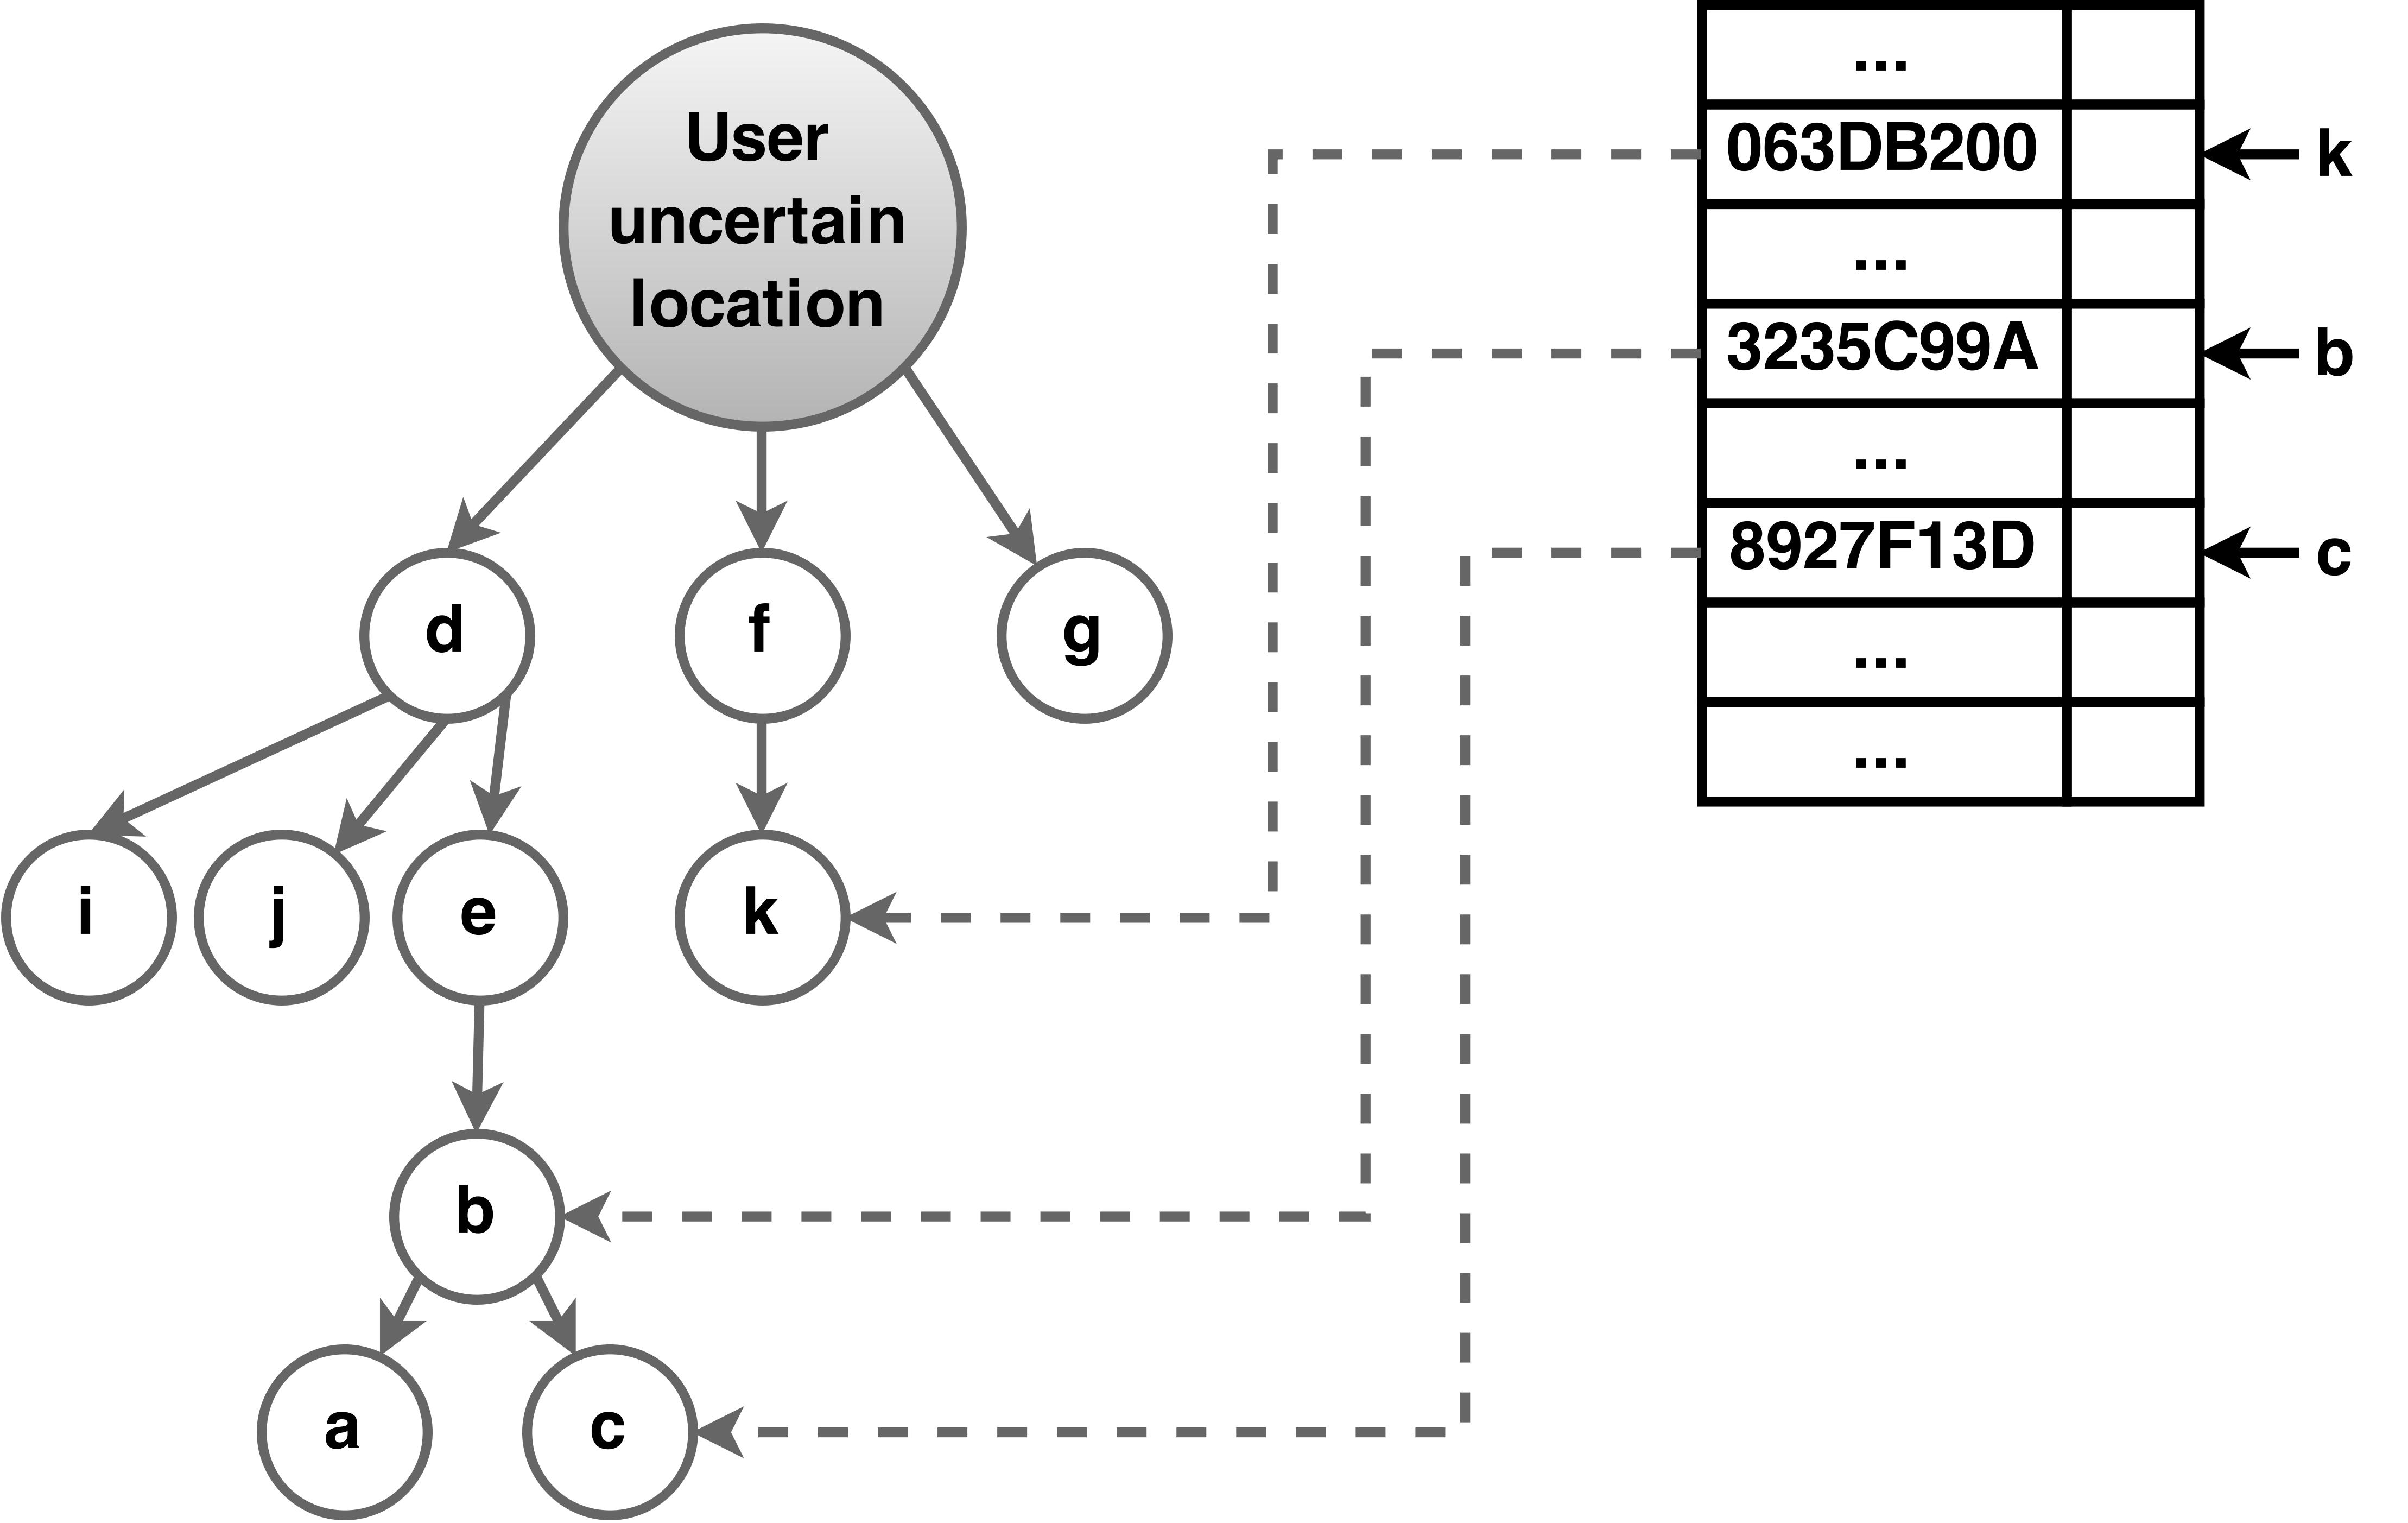
\includegraphics[width=0.5\textwidth]{Hashtable}
  \caption{Hashtable used to optimize node lookup in \pf.}
  \label{fig:hashtable}
\end{figure}

\section {Competitive Algorithm: Time-Parameterized R-Tree (TPR Tree)}
\label{sec:tpr}
The \TPR ~\cite{Saltenis00} is one of the data structure designed for dealing with moving objects under uncertainty. We take such data structure as our baseline for the experiments and in this section we will go briefly over the details of the \TPR prediction algorithm.
\TPR algorithm is given previous uncertainty region $R_A$, current uncertainty region $R_B$ and the next uncertainty region $R_C$ to predict probability $p$ of getting into that region. The algorithm steps are described below:
\begin{itemize}
\item Create vector $v$ from center of $R_A$ to center of $R_B$
\item Find radius $r$ by calculating euclidean distance between center of $R_B$ and $R_C$
\item Construct circle $c$ which have center at $R_B$ and radius $r$
\item Compute intersection points $p_1$ and $p_2$ between vector $v$ and circle $c$ as indicated in \cite{Middleditch88}
\item Calculate distance $d$ which is the max distance from $p_1$ and $p_2$ and center of $R_C$
\item Find number of nodes $count$ within circle that has center at $R_C$ and radius $d$ and return prediction probability $1/count$
\end{itemize}

An visual example that explains the prediction is in Figure \ref{fig:tpr}.

\begin{figure}[ht]
  \centering
    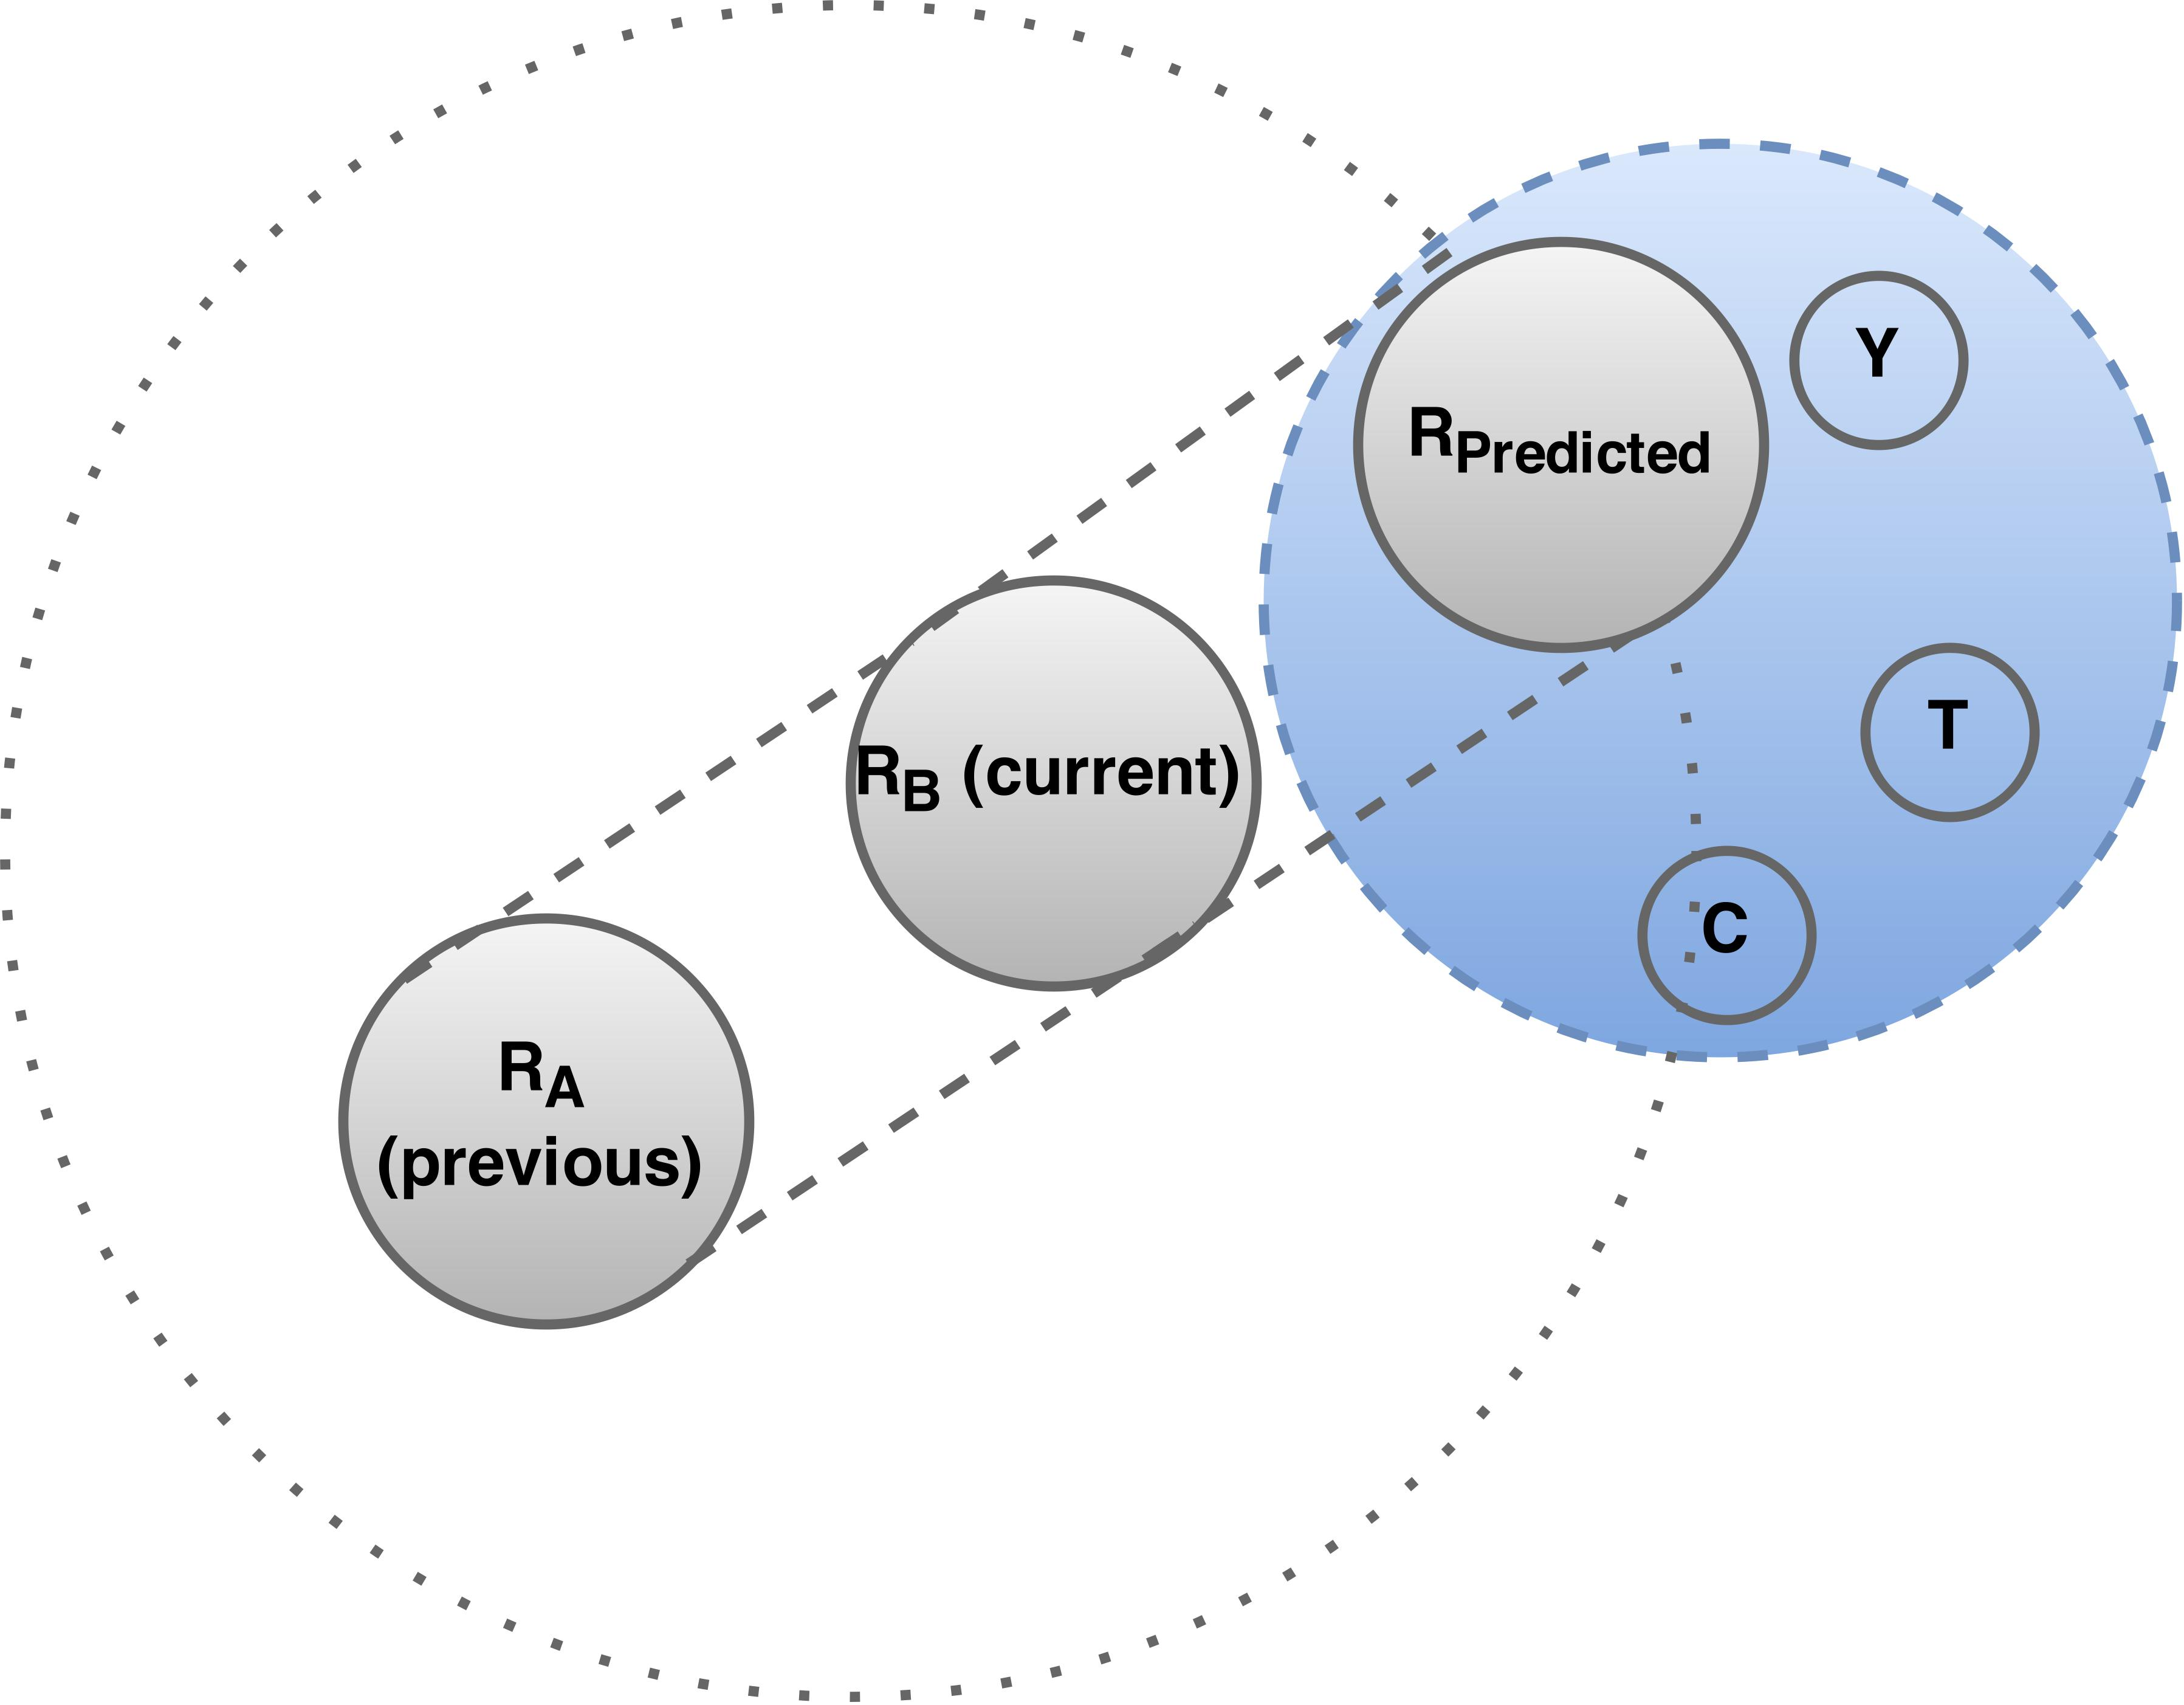
\includegraphics[width=0.5\textwidth]{TPR}
  \caption{TPR Tree Prediction Algorithm.}
  \label{fig:tpr}
\end{figure}